\subsection{Convex Functions}
Let us first give the definition of convex sets.
\begin{definition}[Convex set]
	A set $C$ is convex, if the line segment between any two points in $C$ lies in $C$, i.e., if any $x, y\in C$ and any $\alpha$ with $0\leq \alpha \leq 1$, there holds
	\begin{equation}
	\alpha x+ (1- \alpha)y \in C.
	\end{equation}
\end{definition}
 
%Based on the definition above, we have the next property of convex sets.
%\begin{lemma}
%[Homework] Let $C$ be a convex set, with $x_{1}, \dots, x_{k}\in C$, and let $\alpha_{1}, \dots, \alpha_{k} \in \mathbb{R}$ satisfy $\alpha_{i} \geq 0$ and  $\sum_{i =1}^{k} \alpha_{i} = 1$, then 
%	\begin{equation}
%	\sum_{i = 1}^{k}\alpha_{i}x^{i} \in C,
%	\end{equation}	
%\end{lemma}	

Following the definition of convex set, we define convex function as following.
\begin{definition}[Convex function]
	Let $C \subset \mathbb{R}^n$ be a convex set and $f: C \rightarrow \mathbb{R}$:
	\begin{enumerate}
		\item $f$ is called {\bf convex} if for any $x, y \in C$ and $\alpha\in [0, 1]$
		\begin{equation}
		f(\alpha x + (1- \alpha)y) \leq \alpha f(x )+ (1- \alpha)f(y).	
		\end{equation}
		\item $f$ is called {\bf strictly convex} if for any $x\neq y \in C$ and $\alpha\in (0, 1)$:
		\begin{equation}
		f(\alpha x + (1- \alpha)y) < \alpha f(x ) + (1 - \alpha)f(y).
		\end{equation}
		\item A function $f$ is said to be (strictly) {\bf concave} if $-f$ is (strictly) convex.
	\end{enumerate}
\end{definition}
%With mentioned previously property of convex sets, it is easy to expend the above definition of convex function. Here we write as one lemma without proof. 
%\begin{lemma}
%[Homework]Let $C$ be a convex set, with $x_{1}, \dots, x_{k}\in C$, and let $\alpha_{1}, \dots, \alpha_{k} \in \mathbb{R}$ satisfy $\alpha_{i} \geq 0$ and  $\sum_{i =1}^{k} \alpha_{i} = 1$, then 
%	\begin{equation}
%	f(\sum_{i = 1}^{k}\alpha_{i}x_{i}) \leq \sum_{i = 1}^{k}\alpha_{i}f(x_{i}) .
%	\end{equation}	
%\end{lemma}
Fig. \ref{convexfunc} and \ref{nonconvexfunc} are diagrams  for convex function definition.
\begin{figure}[H]
\centering                    % 大图名称
\subfigure[Convex function]{                    %第二张子图
\begin{minipage}{4cm}\centering
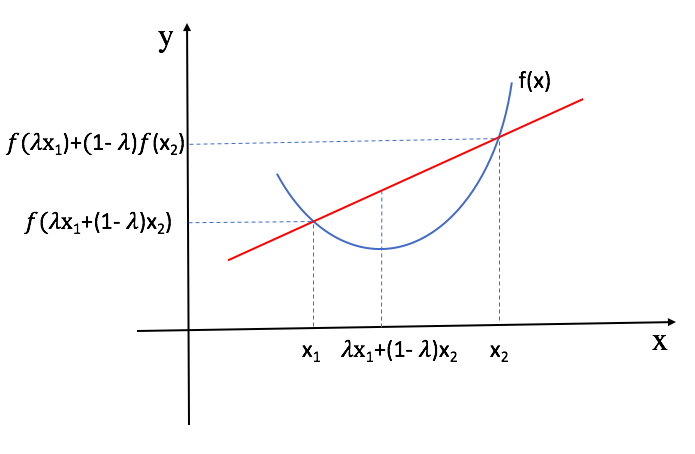
\includegraphics[width=1\textwidth] {6DL/figures/convexfunction.png}\label{convexfunc}
\end{minipage}   }  
 \quad
 \subfigure[Nonconvex function]{                    %第二张子图
\begin{minipage}{4cm}\centering
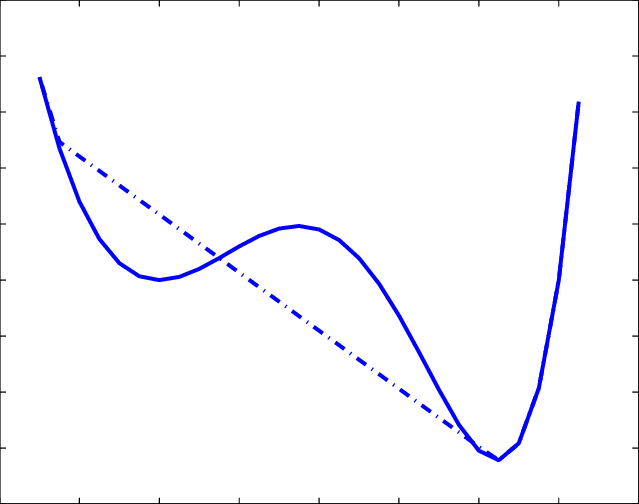
\includegraphics[width=1\textwidth,height=0.8\textwidth] {6DL/figures/nonconvexfunction.png}\label{nonconvexfunc}
\end{minipage}   }  
\caption{Convex and nonconvex functions} %     
\end{figure}



\begin{lemma}
	If $f(x)$ is differentiable on $\mathbb{R}^n$, then $f(x)$ is convex if and only if
	\begin{equation}
	f( x) \ge f( y) + \nabla f( y)\cdot ( x -  y), \forall x, y \in \mathbb{R}^n.
	\end{equation}
\end{lemma}
Based on the lemma, we can first have  Fig. \ref{fig:convextangent} for convex functions, namely, the curve of a convex function is always above the tangent lines.
\begin{figure}[H]
\centering
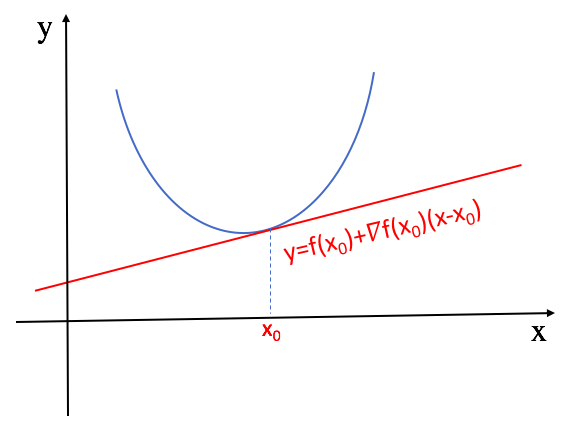
\includegraphics[width=.5\textwidth] {6DL/figures/convextangent.png}
\caption{Tangent line of a convex function}
\label{fig:convextangent}
\end{figure}

\begin{proof}
	Let $z=\alpha x+(1-\alpha )y, 0\leq \alpha \leq 1, \forall x,y \in \mathbb{R}^n$, we have these next two Taylor expansion:
	\begin{equation}\label{key}
	\begin{aligned}
	&f(x)\geq f(z)+ \nabla f(z)(x-z),\\
	&f(y)\geq f(z)+ \nabla f(z)(y-z).
	\end{aligned}
	\end{equation}
	Then we have
	\begin{equation}
	\begin{aligned}
	\alpha f(x) + (1-\alpha) f(y)
	\geq &f(z) + \nabla f(z)[\alpha(x-z)+(1-\alpha)(y-z)]\\
	=&f(z)
	=f(\alpha x +(1-\alpha)y).
	\end{aligned}
	\end{equation}
	Thus we have
	\begin{equation}\label{key}
	\alpha f(x) + (1-\alpha) f(y) \ge f(\alpha x +(1-\alpha)y).
	\end{equation}
	This finishes the proof.
	
	On the other hand if	$f(x)$ is differentiable on $\mathbb{R}^n$, then 
	$$
	f( x) \ge f( y) + \nabla f( y)\cdot ( x -  y), \forall x, y \in \mathbb{R}^n
	$$ 
	if $f(x)$ is convex.
\end{proof}

\begin{definition}[$\lambda$-strongly convex]\label{def:strongconvex}
We say that $f(x)$ is $\lambda$-strongly convex if
	\begin{equation}\label{equ:lambdastronglyconvex}
	f(x)  \ge f(y) + \nabla f(y)\cdot(x-y) + \frac{\lambda}{2}\|x-y\|^2, \quad \forall x, y \in C,
	\end{equation}
	for some $\lambda >0$.
\end{definition} 
\begin{lemma}
Let $\sigma(\nabla^2f)$ be the spectrum of the operator $\nabla^2 f$. If
$$
\sigma(\nabla^2f)\subset [\lambda, L],
$$ 
then the condition \eqref{equ:lambdastronglyconvex} holds.
\end{lemma}

\begin{lemma} 
If $f(x)$ is $\lambda$-strongly convex,
	\begin{equation}\label{strongConvIneq}
		\nabla f(x)\cdot(x - x^*) \ge f(x) - f(x^*) +\frac{\lambda}{2}\|x - x^*\|^2\ge \lambda \|x - x^*\|^2.
		\end{equation} 
\end{lemma}

\begin{example}
	Consider $f(x) = \|x\|^2$, then we have
	\begin{equation}\label{key}
	\frac{\partial f}{\partial x_{i}}=2x_{i}, \nabla f = 2x \in R^n,\quad \nabla^2f=2I_{n\times n}\in\mathbb{R}^{n\times n}.
	\end{equation}
	So, we have $\lambda_{\rm min}(\nabla^2f)=2>0$ and
	\begin{equation}
	\begin{aligned}
	f(x)-f(y)-\nabla f(y)(x-y)
	=&\left \| x \right \|^2-\left \| y \right \|^2-2y(x-y)\\
	=&\left \| x \right \|^2-\left \| y \right \|^2-2xy+2\left \| y \right \|^2\\
	=&\left \| x \right \|^2-2xy+\left \| y \right \|^2\\
	=&\left \| x-y \right \|^2\\
	=&\frac{\lambda }{2}\left \| x-y \right \|^2 , \quad \lambda=2.
	\end{aligned}
	\end{equation}	
	Thus, $f(x) = \|x\|^2$ is 2-strongly convex
\end{example}
\begin{lemma}
If $f(x)$ is $\lambda$-strongly convex and $\lambda(\nabla^2 f)\le L$, then
$$
\lambda\|x-y\|\le \|\nabla f(x) - \nabla f(y)\|\le L\|x-y\|.
$$
\end{lemma}
\begin{assumption}\label{ass:GD}
We make the following assumptions:
\begin{enumerate}
	\item $f(x)$ is $\lambda$-strongly convex for some $\lambda >0$ with the definition in Definition \ref{def:strongconvex}.  
	\item $\nabla f$ is $L$-Lipschitz, i.e., 
	\begin{equation}\label{key}
	\|\nabla f(x) - \nabla f(y)\| \le L\|x - y\|, \forall x,y.
	\end{equation}
\end{enumerate}	
\end{assumption}
\begin{example}
Actually, the loss function of the logistic regression model 
	\begin{equation}\label{key}
	L(\theta) = -\log P(\theta),
	\end{equation}
	is a convex  function of $\theta$. 
	Furthermore, the loss function of the regularized logistic regression model 
	\begin{equation}\label{key}
	L_\lambda(\theta) = -\log P(\theta) + \lambda \|\theta\|_F^2, \lambda > 0
	\end{equation}
	  is a $\lambda'$-strongly convex function of $\theta$($\lambda'$ is related to $\lambda$).
\end{example}

We also have these following interesting properties of convex function. 

\begin{proposition}[basic properties of convex function] 
	\begin{enumerate}
		\item If $f(x)$, $g(x)$ are both convex, then $\alpha f(x) + \beta g(x)$ is also convex, if $\alpha, \beta \geq 0$.
		\item  Linear function is both convex and concave. Here, $f(x)$ is concave if and only if $-f(x)$ is convex.
		\item If $f(x)$ is a convex function on $\mathbb{R}^n$, then $g(y) = f(Ay+b)$ is a convex function on $\mathbb{R}^m$. Here $A \in \mathbb{R}^{m \times n}$ and $b\in \mathbb{R}^m$. 
		\item  If $g(x)$ is a convex function on $\mathbb{R}^n$, and the function $f(u)$ is convex function on $\mathbb{R}$ and non-decreasing, then the composite function $f \circ g(x) = f(g(x))$ is convex.
	\end{enumerate}
\end{proposition}
The proof is straightforward and left to the interested readers.

\begin{theorem}[Jensen's inequality]
If $p_1, \cdots, p_n$ are positive numbers which sum to 1 and $f$ is a real continuous function which is convex, then
$$
f(\sum_{i=1}^n\alpha_ix_i)\le \sum_{i=1}^n \alpha_if(x_i).
$$
If $f$ is concave, then
$$
f(\sum_{i=1}^n\alpha_ix_i)\ge \sum_{i=1}^n \alpha_if(x_i).
$$
\end{theorem}
